%************************************************
\chapter{Introduction, context and aims}\label{ch:Intrd}
%************************************************

Along this work, we are going to perform a deep study of the geodesic movement of free fall particles in the Kerr spacetime. The Kerr spacetime describes what is known as a rotating black hole. Some examples of popular black holes are the supermassive black holes located at the center of the active galaxies, or the intermediate mass black holes, which are the bridge between stellar mass black holes and supermassive black holes, and its existence is still a mystery. Using the solution to the motion of test particles we can explain many purely relativistic effects such as the precession of the perihelion of Mercury and the deflection of light rays as they pass close to a massive object. Thus, the motion of test particles in the Kerr spacetime conforms not only a way to understand more thoroughly relativistic phenomena but also determines important information for the detection and prediction of relevant astrophysical objects as pulsars (which are highly magnetized rotating neutron star that emits a beam of electromagnetic radiation) and quasars. Therefore, the understanding and the study of motion around Kerr black holes helps us to understand their nature in more detail. Solutions to the motion of particles in this spacetime are commonly difficult to understand and categorize and there are entire books dedicated to this task. There are a lot of definitions of what a black hole is. The physical definition of a black hole is "a region of spacetime from which gravity prevents anything, including light, from escaping''.
\begin{figure}[b!]
\centering
\begin{tabular}{c}
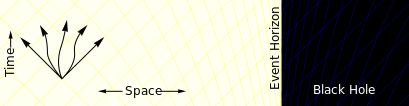
\includegraphics[width=0.7\textwidth]{img/Introd/1.png}\\
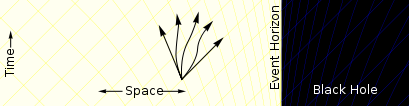
\includegraphics[width=0.7\textwidth]{img/Introd/2.png}\\
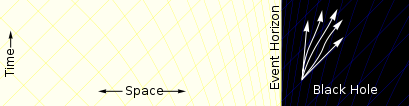
\includegraphics[width=0.7\textwidth]{img/Introd/3.png}
\end{tabular}
\caption{The figure shows how particles can move in any direction outside the event horizon but they can only move inwards the black hole once the event horizon is crossed.}
\label{blackholecones}
\end{figure}
The mathematically accurate version of this definition is more technical and involves the existence of a \textit{spacetime singularity}, which is a region of the spacetime where the movement of the particles that reaches this area cannot be extended, and an \textit{event horizon}, which is a surface that has the property to prevent the particles that cross this region to go back. We can understand this behavior with the use of the Minkowsky diagrams, that are plots in which the time coordinate is represented in the vertical axis and the space coordinate is represented in the horizontal axis. In these diagrams the trajectories of the photons are straight lines sloping at 45 degrees. As photons (null particles onwards) are the limit behavior of mass particles (timelike particles onwards), the last ones must remain inside the cone defined by the straight lines at 45 degrees. This is known as the ''light cone'' and can be used to study the regions of the spacetime that are accessible to physical particles (causal particles onwards). As we can see in \cref{blackholecones}, the light cones outside the event horizon allow causal particles to move in any direction, but closer to the horizon the spacetime starts to deform. There are more allowed movements going towards the horizon than moving away. Inside the event horizon causal particles are not allowed to escape from this region, as the spacetime is so bended that the only allowed behavior is moving towards the black hole. 

The black holes can be categorized in virtue of the ''no hair theorem'', which stipulates that these entities can be described with three properties: Mass, electromagnetic charge and angular momentum. With this information in mind, the black holes are named as
\begin{figure*}[hpt!]
\centerline{
\begin{tabular}{c|c|c}
 & Non-rotating ($L=0$) & Rotating ($L\neq0$) \\   \hline
 Uncharged ($Q=0$) & Schwarzschild &  Kerr \\   \hline
 Charged ($Q \neq 0$) & Reissner Nordstr\"om & Kerr-Newman
\end{tabular}
}
\end{figure*}

The complexity order is 
\begin{equation*}
 \text{Schwarzschild }\rightarrow \text{Reissner Nordstr\"om} \rightarrow \text{Kerr} \rightarrow \text{Kerr-Newman}.
\end{equation*}
As general relativity states, freefall particles in the spacetime must move along causal (timelike or lightlike) \textit{geodesics}, and therefore in order to understand the paths of these particles we must obtain and analyze the geodesics trajectories of the spacetime. In the \gls{SW} spacetime, the geodesic flow is well understood but its study still provides new and interesting results \cite{belbruno2011dynamical,marck1996short,galindo2014mcgehee}. In the \gls{RN} spacetime, the geodesic flow is much more complicated due to the fact that the spacetime structure is more complex and some features of the geodesics are still being analyzed nowadays \cite{galindo2014mcgehee}.
\begin{figure}[htp!]  
\begin{center}
 \centerline{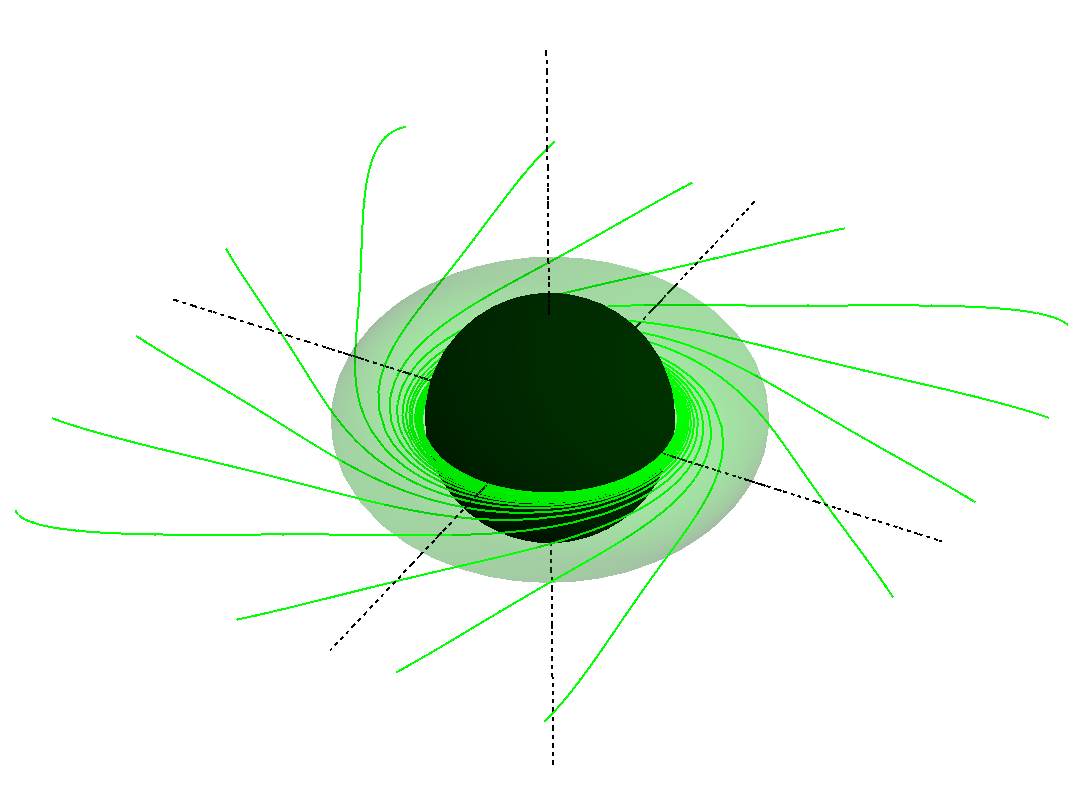
\includegraphics[width=0.8\textwidth]{img/Introd/ZAMOS.png}}
 \end{center}
 \vspace{-1.5cm}
 \caption{Trajectories with zero angular momentum in the Kerr spacetime.}
 \label{fig:rotzam}
\end{figure}
The study of the Kerr spacetime is even more complex that in the \gls{RN} spacetime and the geodesic flow is very difficult to understand and analyze. Indeed, there are very intricate technical books dedicated to this topic \cite{o1995geometry} that do not even provide a general (either quantitatively or qualitatively) description for all possible geodesics. Due to its complexity, the Kerr metric is still an important research field because it is known that the spacetime described by every collapsing astrophysical object approaches the Kerr spacetime asymptotically, and therefore almost every black hole in the universe is a Kerr black hole (except those which also have charge, but as the charge is very low for common astrophysical objects). It is interesting to note that while the \gls{SW} and \gls{RN} geometries can be used to describe the exterior of a spherically symmetric object in virtue of the Birkhoff theorem \cite{birkhoff1923relativity}, the Kerr geometry only describes a black hole. For example, it is known that while the spacetime singularities in the \gls{SW} and \gls{RN} geometries are single points (that for mathematical reasons are not in the spacetime), the Kerr singularity is a topological ring. Also, one of the most popular features in the Kerr geometry is the \textit{frame dragging}. This phenomenon consists in the Kerr black hole dragging the fabric of spacetime itself in its movement and therefore, it also drags the trajectory of the physical particles moving in its presence. This effect can be so relevant, that there are some regions in the black hole known as \textit{ergoregions} where all the particles are forced to rotate in the same direction as the black hole does. Indeed, trajectories with zero angular momentum (that in the \gls{SW} and \gls{RN} spacetimes correspond to straight lines) are not straight lines but curved trajectories that spin co-rotating with the black hole as is depicted in \cref{fig:rotzam}.
\begin{figure}[hpt!]  
\begin{center}
 \centerline{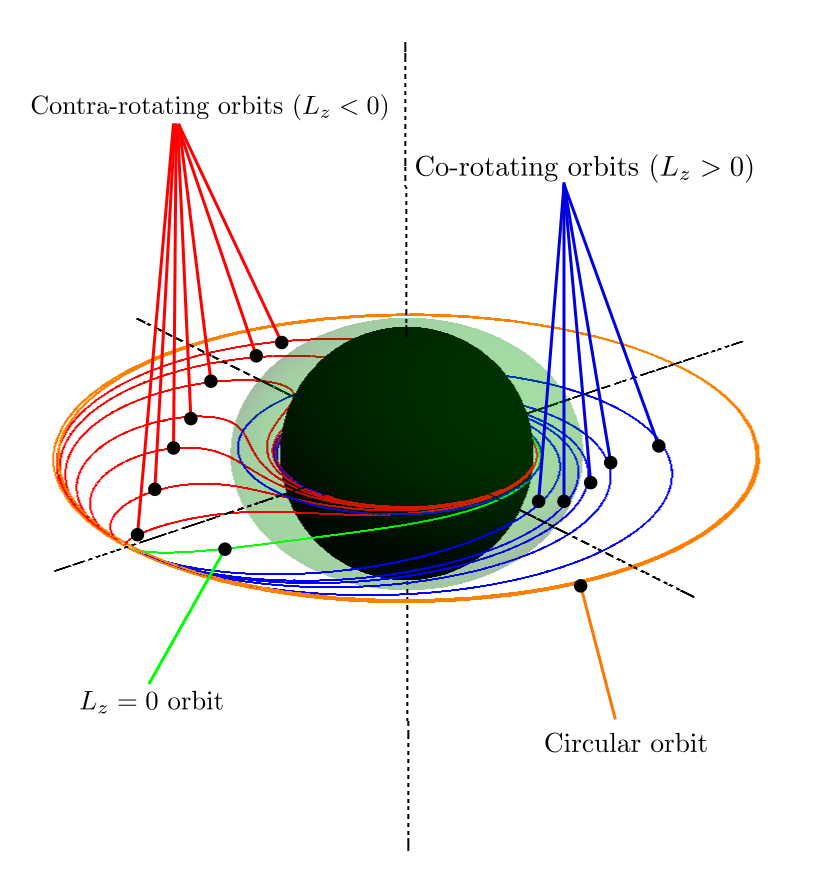
\includegraphics[width=0.7\textwidth]{img/Introd/Orbits.png}}
 \end{center}
 \vspace{-1.5cm}
 \caption{Behavior of timelike particles near a Kerr black hole. The black hole is rotating anticlockwise. The black region correspond to the event horizon while the green one correspond to the ergoregion. The orbits drawn red are retrograde geodesic that are spin-reversed by the black hole, the blue paths are direct geodesics, the orange curve is a circular orbit while the green one is the $L_z=0$ geodesic.}
 \label{fig:orbits}
\end{figure} 
All the possible behaviors are depicted in \cref{fig:orbits} where we can see how trajectories attempting to enter the ergoregion contra-rotating with respect to the black hole, are forced to spin in the same direction of the black hole. Also, particles with zero angular momentum are still moving in a co-rotating movement as well as particles with positive angular momentum. As also happens in the \gls{SW} and \gls{RN} geometries, particles with enough angular momentum can move in circular orbits around the Kerr black hole.

But there are features of the Kerr black holes even stranger than the frame dragging. The Kerr black hole has what is known as a Einstein - Rosen bridge or more typically as a \textit{wormhole}, which is a topological feature of the spacetime that connects two different regions (called sometimes ''universes'' in the literature) of the spacetime. In this case, the wormhole (which is located at the center of the ring singularity) leads to the \textit{negative space}, a region of the spacetime in which gravity is repulsive. In this space there also causal violations, i.e. there exist trajectories allowed to physical particles that lead to time travel. As the wormhole is inside the event horizon, these trajectories cannot be seen from outside the black hole. Thus, possible causality violations are ''protected'' by the event horizon. The maximal analytic extension of the Kerr black hole (which is the whole spacetime described by the Kerr metric) is even more complex and reveals that the Kerr black hole has an infinite amount of asymptotically flat regions and an infinite amount of wormholes that connects them. These wormholes are different from the wormholes that connect with the negative space.

As we can see, the structure of the spacetime is very complex and therefore, the description of the movement of physical particles in the Kerr geometry is very difficult to understand. The aim of this work is present a method that allows us to analyze the full motion of the particles in some regions of interest in the spacetime. Our main focus will be the use of dynamical systems, which have proven to be a powerful tool in the study and description of physical systems, as demonstrated by theoretical mechanics. The combination of General Relativity and dynamical systems is a very novel approach to the problem \cite{stoica1997schwarzschild,belbruno2011dynamical,galindo2014mcgehee} which describes certain known results from a completely new perspective. The two regions in which we are interested are the axis of symmetry and the equatorial plane. The axis of symmetry is a very important region because it contains the easiest way to travel to the negative space. The description of the geodesic flow in the axis of symmetry is a very difficult topic with the standard methods because a complete study of the geodesic flow involves the movement in an infinite amount of asymptotically flat regions and negative spaces. This is the reason why the current analysis of the geodesic flow in the axis is very difficult to understand and why it had remained incomplete. In this work, we achieve to describe the whole geodesic flow in the axis of symmetry by the use of a dynamical system technique that projects all the different trajectories into one two-dimensional phase portrait. This is a great simplification of this problem. The other region in which we are interested is in the equatorial plane, because it contains the ring singularity of the Kerr spacetime and the disk inside this singular ring, which is the wormhole that connects to the negative space. The analysis of the trajectories in the axis and in the equatorial plane is essential because allows us to understand some very important characteristics of the black holes as the jets or accretion disks. What is known as the Penrose process conforms a mechanism that allows us to understand the powerful jets that quasars and rotating black holes emit. This process involves expelled particles that gain energy while the black hole loses it, decreasing its own rotation. This is still one of many viable competing models for quasar jets.

Its important to warn that the Kerr metric describes an \textit{eternal black hole}, which has existed forever and therefore does not come from a collapsing astrophysical object. It is known that the Kerr black holes produced by the gravitational collapse probably will not have the infinite wormhol structure, as these wormholes are unstable and will collapse under small perturbations. However, the wormhole that leads to negative space is stable and probably will survive the gravitational collapse.

This work is organized as follows: In \cref{ch:KerrG} we present a brief but concise description of the Kerr spacetime and its main features. As we will see in this chapter we will need a new coordinate system that allow us to describe the geodesic flow in the whole spacetime without having to worry about  horizons or wormholes. In \cref{ch:introduction} we define the new coordinate system and we express all the quantities of interest in this new coordinates. Also, we show how the Kerr spacetime is described in the new coordinates and the main features of the important surfaces. In \cref{ch:MAE} perform a rigorous analysis of the topological identification describing the wormhole that lead to the negative space and we also describe how the new coordinates are very useful studying the movement in maximal extension, which is also examined in detail. In \cref{ch:dinamicsys} we performed a comprehensive study of the geodesic flow along the axis of symmetry in terms of dynamical systems, with particular attention to the causal structure and the stability of the motion along the axis. After that, a similar study about the equatorial plane is performed in \cref{ch:ep} with special emphasis in the disk inside the singular ring and its stability. Finally in \cref{ch:nsog} we display some interesting geodesic defined along the whole Kerr spacetime obtained by a numerical integration software developed for this work. Some useful information that completes the understanding of this work can be found in \cref{Killingchapter}.
